\section{Auswertung}
\subsection{Vorverstärkte Pulse auf dem Oszilloskop}
Die Pulse des Surface-Barrier Detektors werden vorverstärkt und einmal mit und einmal ohne Amplifier auf dem Oszilloskop dargestellt.
In den Abbildungen \ref{fig:2} und \ref{fig:1} werden die Pulse gegen die Zeit aufgetragen.

\begin{figure}[H]
  \centering
  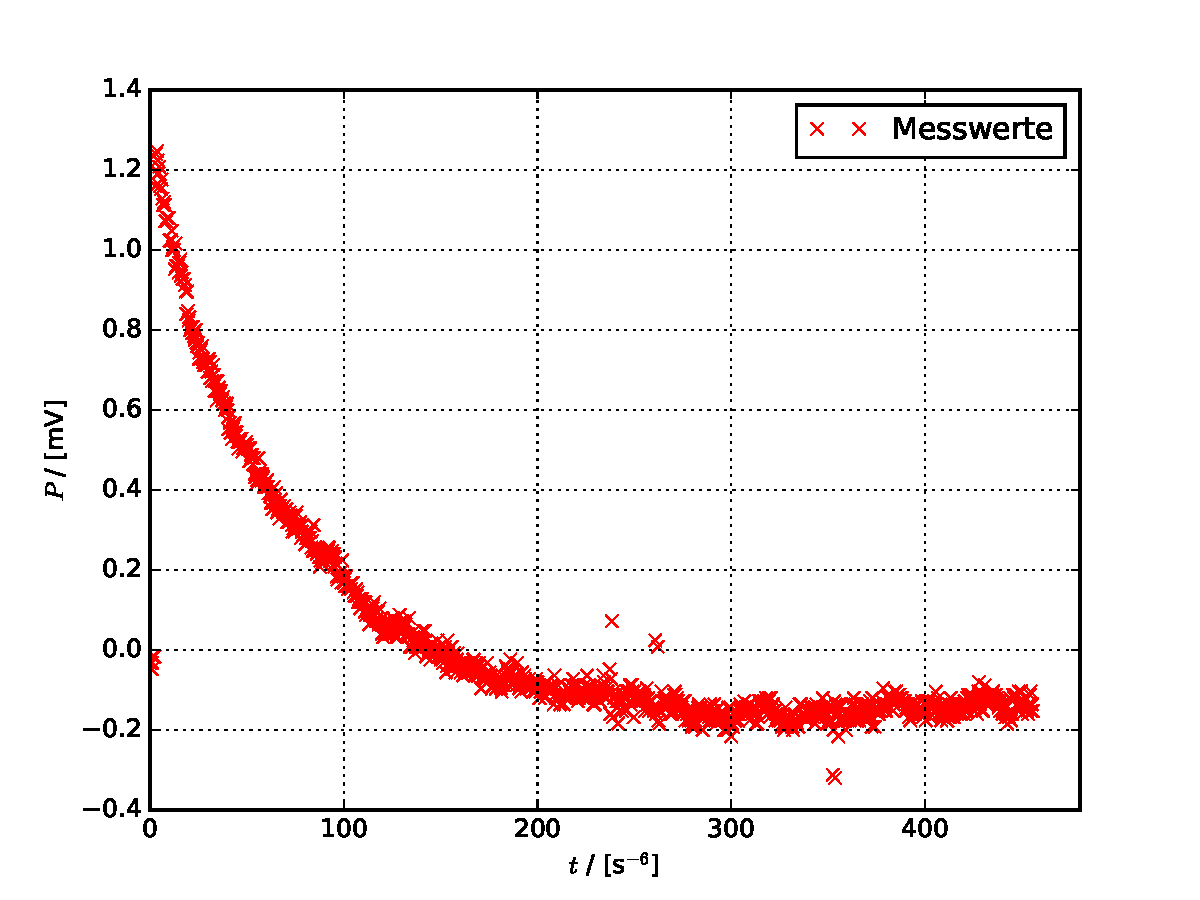
\includegraphics[width=\textwidth]{osz2.pdf}
  \caption{Pulse in Abhängigkeit von der Zeit ohne angeschlossenem Amplifier.}
  \label{fig:2}
\end{figure}

Ohne angeschlosseem Amplifier schwankt der Wert vor dem Puls um $0\,\text{V}$.
Danach steigt der Puls mit einer Anstiegszeit von $0\,\si{\micro\second}$ auf ca. $1,25\,\text{mV}$.
Mit einem "Überschwinger" pendelt sich der Wert wieder auf ca. $0\,\text{V}$ ein.

\begin{figure}[H]
  \centering
  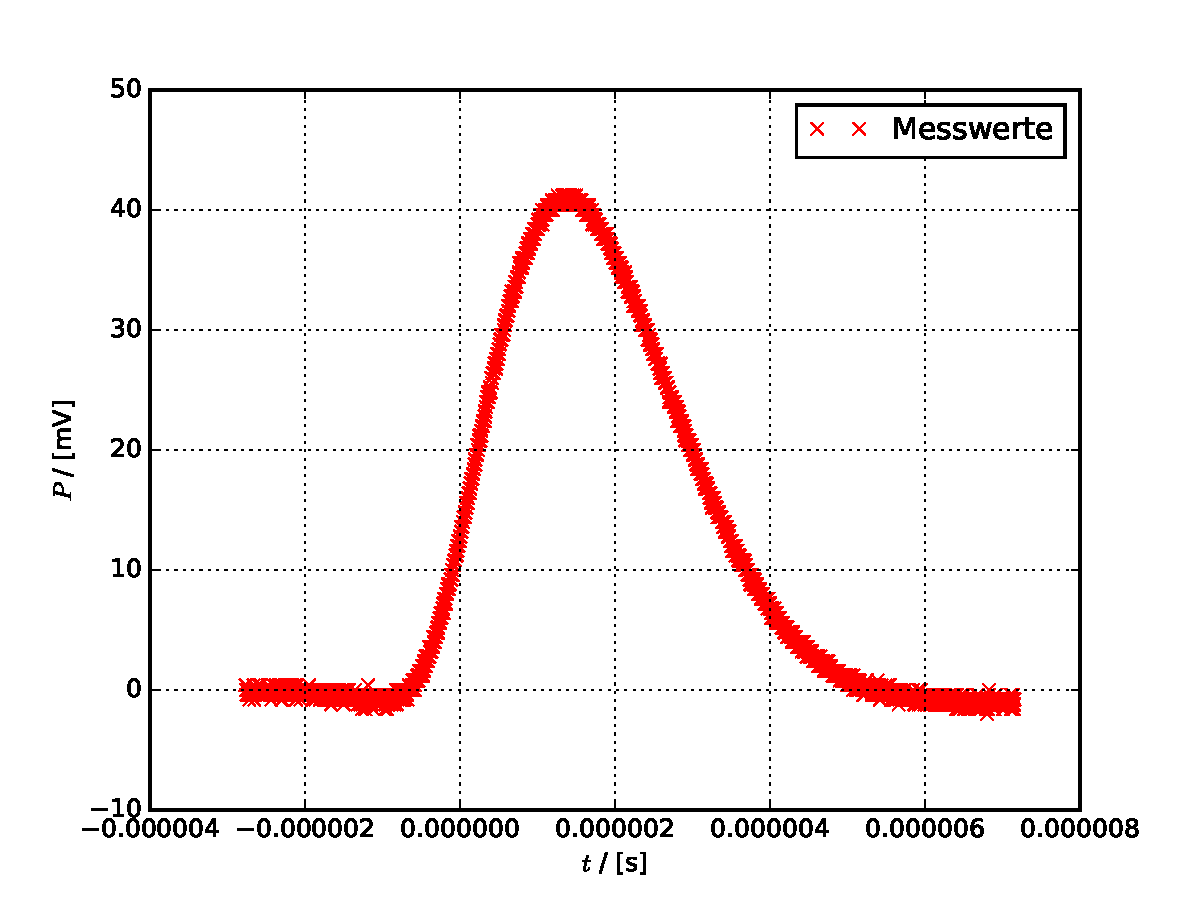
\includegraphics[width=\textwidth]{osz1.pdf}
  \caption{Pulse in Abhängigkeit von der Zeit mit angeschlossenem Amplifier.}
  \label{fig:1}
\end{figure}

Die Anstiegszeit mit angeschlossenem Amplifier beträgt ca. $8\,\si{\micro\second}$.
Der Puls steigt von $0\,\text{mV}$ auf ca. $41\,\text{mV}$ und fällt wieder auf seinen Ursprungswert ab.

\subsection{Bestimmung der Goldfoliendicke}
In Tabelle \ref{tab:U(p)} sind die Messwerte für die Pulshöhen des Detektors in Abhängigkeit vom Kammerdruck zu entnehmen.

\begin{table}[H]
  \centering
  \begin{tabular}{cc|cc}
    \toprule
    \multicolumn{2}{c}{Mit Goldfolie} & \multicolumn{2}{c}{Ohne Goldfolie} \\
    Pulshöhe [V] & Druck [mbar] & Pulshöhe [V] & Druck [mbar] \\
    \midrule
    1.020 & 0.025 & 1.310 & 0.075 \\
    0.936 & 0.639 & 1.260 & 0.290 \\
    0.896 & 7.900 & 1.210 & 51.20 \\
    0.832 & 18.30 & 1.140 & 84.90 \\
    0.752 & 38.00 & 1.050 & 110.5 \\
    0.632 & 61.10 & 0.928 & 126.6 \\
    0.512 & 109.1 & 0.856 & 141.6 \\
    0.680 & 95.70 & 0.728 & 157.5 \\
    0.800 & 75.60 & 0.672 & 174.6 \\
    0.840 & 57.20 & 0.904 & 136.9 \\
    0.984 & 45.00 & 1.010 & 116.0 \\
    1.000 & 21.50 & 1.120 & 93.30 \\
    1.090 & 1.500 & 1.180 & 74.00 \\
    \bottomrule
  \end{tabular}
  \caption{Puls in Abhängigkeit vom Kammerdruck.}
  \label{tab:U(p)}
\end{table}

In Abbildung \ref{fig:U(p)} sind die Pulse in Abhängigkeit vom Kammerdruck aufgetragen.
Außerdem wird eine Ausgleichsrechnung der Form $y=ax+b$ durchgeführt.

\begin{figure}[H]
  \centering
  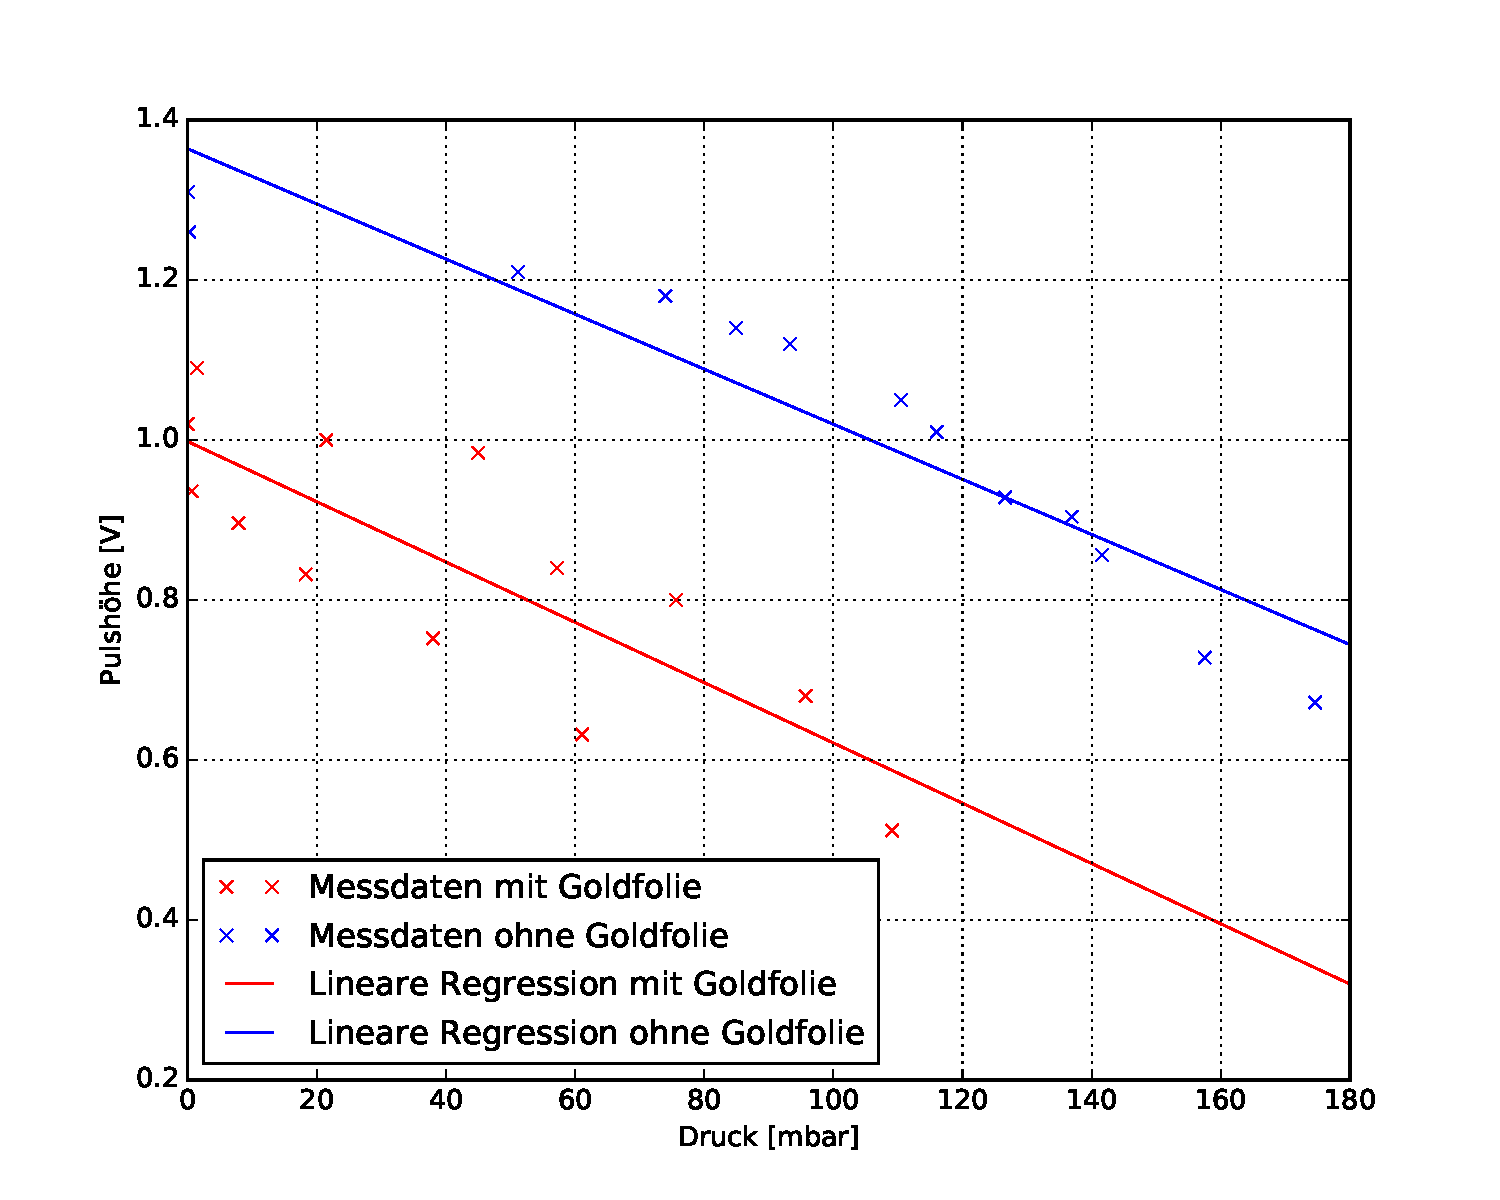
\includegraphics[width=\textwidth]{pulshohe_druck2.pdf}
  \caption{Pulse in Abhängigkeit vom Druck mit und ohne Goldfolie und lineare Regression beider Messreihen.}
  \label{fig:U(p)}
\end{figure}

Für die Parameter folgt
\begin{gather*}
  \textcolor{red}{a_1 = (-0,0038 \pm 0,0008)\,\frac{\text{V}}{\text{mbar}}}, \\
  \textcolor{red}{b_1 = (1,00 \pm 0,04)\,\text{V}}, \\
  \textcolor{blue}{a_2 = (0,0034 \pm 0,0004)\,\frac{\text{V}}{\text{mbar}}}, \\
  \textcolor{blue}{b_2 = (1,36 \pm 0,04)\,\text{V}}.
\end{gather*}
Der $y$-Achsenabschnitt $b_2$ der Messreihe ohne Goldfolie gibt an,
wie hoch die Energie eines Alphateilchens im Vakuum ist.
Der Abbildung \ref{fig:amnp} kann entnommen werden,
dass die mittlere kinetische Energie des $\alpha$-Teilchens $E_{\alpha} = 5,48\,\text{MeV}$ beträgt.
Somit entspricht die Pulshöhe der mittleren kinetischen Energie des $\alpha$-Teilchens:
\begin{align}
  b_2 = 1,36 \propto E_{\alpha} = 5,48\,\text{MeV}.
  \label{eqn:bE}
\end{align}
Mit diesem Wissen kann der Energieverlust berechnet werden.
Der Pulsverlust ist gegeben durch
\begin{equation}
  \Delta{P} = b_2-b_1.
\end{equation}
Der Fehler beträgt unter Berücksichtigung der Gaußschen Fehlerfortpflanzung
\begin{equation}
  \Delta(\Delta{P}) = \sqrt{(1-b_1)^2\cdot(\Delta{b_2})^2 + (b_2-1)^2\cdot(\Delta{b_1})^2}.
\end{equation}
Somit ist ergibt sich
\begin{align*}
  \Delta{P}\pm\Delta(\Delta{P}) = (0,36\pm0,06)\,\text{V}
\end{align*}
Durch den proportionalen Zusammenhang \eqref{eqn:bE} ergibt sich aus dem Pulsverlust der Energieverlust
\begin{align*}
  \Delta{E} = \frac{E_{\alpha}}{b_2}\cdot{\Delta{P}} = (1,45\pm0,25)\,\text{MeV}.
\end{align*}

\subsection{Bestimmung des differentiellen Wirkungsquerschnitts}

\subsection{Untersuchung des Einflusses der Mehrfachstreuung}

\subsection{Messung der Z-Abhängigkeit an einer }
